\documentclass[onecolumn, draftclsnofoot,10pt, compsoc]{IEEEtran}
\usepackage{graphicx}
\usepackage{url}
\usepackage{setspace}
\usepackage{pgfgantt}

\usepackage{geometry}
\geometry{textheight=9.5in, textwidth=7in}

% 1. Fill in these details
\def \CapstoneTeamName{        Team 25}
\def \CapstoneTeamNumber{        25}
\def \GroupMemberOne{            Lazar Sharipoff}
\def \GroupMemberTwo{            Jordan Davis}
\def \GroupMemberThree{            Glen Anderson}
\def \CapstoneProjectName{        Smart Home Intercom System}
\def \CapstoneSponsorCompany{    Oregon State EECS}
\def \CapstoneSponsorPerson{        D. Kevin McGrath}

% 2. Uncomment the appropriate line below so that the document type works
\def \DocType{        %Problem Statement
                %Requirements Document
                %Technology Review
                Design Document
                %Progress Report
                }
\newcommand\tab[1][1cm]{\hspace*{#1}}            
\newcommand{\NameSigPair}[1]{\par
\makebox[2.75in][r]{#1} \hfil     \makebox[3.25in]{\makebox[2.25in]{\hrulefill} \hfill        \makebox[.75in]{\hrulefill}}
\par\vspace{-12pt} \textit{\tiny\noindent
\makebox[2.75in]{} \hfil        \makebox[3.25in]{\makebox[2.25in][r]{Signature} \hfill    \makebox[.75in][r]{Date}}}}
% 3. If the document is not to be signed, uncomment the RENEWcommand below
\renewcommand{\NameSigPair}[1]{#1}

%%%%%%%%%%%%%%%%%%%%%%%%%%%%%%%%%%%%%%%
\begin{document}
\begin{titlepage}
\pagenumbering{gobble}
\begin{singlespace}
    %\includegraphics[height=4cm]{coe_v_spot1}
\hfill
% 4. If you have a logo, use this includegraphics command to put it on the coversheet.
%\includegraphics[height=4cm]{CompanyLogo}
\par\vspace{.2in}
\centering
\scshape{
\huge CS Capstone \DocType \par
{\large\today}\par
\vspace{.5in}
\textbf{\Huge\CapstoneProjectName}\par
\vfill
{\large Prepared for}\par
\Huge \CapstoneSponsorCompany\par
\vspace{5pt}
{\Large\NameSigPair{\CapstoneSponsorPerson}\par}
{\large Prepared by }\par
Group\CapstoneTeamNumber\par
% 5. comment out the line below this one if you do not wish to name your team
\CapstoneTeamName\par
\vspace{5pt}
{\Large
\NameSigPair{\GroupMemberOne}\par
\NameSigPair{\GroupMemberTwo}\par
\NameSigPair{\GroupMemberThree}\par
}
\vspace{20pt}
}
\begin{abstract}
% 6. Fill in your abstract
The design choices for the Smart Home Intercom System are described in this document in the context of client requirements and the intended purpose of the project. On a high level, the hardware, software, and interface design for this project are discussed. Specifically, each of these sections describes design choices for each part of the system, how the project will be implemented, and the order each part needs to be implemented in. 
\end{abstract}
\end{singlespace}
\end{titlepage}
\newpage
\pagenumbering{arabic}
\tableofcontents
% 7. uncomment this (if applicable). Consider adding a page break.
%\listoffigures
%\listoftables
\clearpage


% 8. now you write!
\section{Introduction}
The Smart Home Intercom System project involves implementing a functional prototype of a system that allows users to communicate between rooms in a home. This document describes the methods that will be used to implement each piece of this project to ensure that the development is well planned, as well as rough timelines where they are appropriate. The document also explains the logical order of development, as certain pieces of the project will need to be done before others can begin.

\section{Scope}
The final project should comprise of a functional prototype of the system along with documentation that will allow others to expand the project easily. The project will include configuring hardware to function with the Raspberry Pi 3, as well as compatible software that implements the requirements of the system. 

\section{Purpose}
This project is intended as a proof of concept for a smart home intercom system. It would allow users to communicate between rooms securely, using audio and video. The system would also include features to make such communication more convenient, such as tracking which room a person was last in and serving as a baby monitor in certain modes. 

\section{Context}
The “Smart Home Intercom System” is built using nodes comprising several pieces of hardware that talk to various parts of a software system to stream video and audio between nodes, along with other features. The system will be used within a home to communicate securely between rooms, without connection to an external network. 

%UML Diagram
\begin{figure}[ht]
\centering
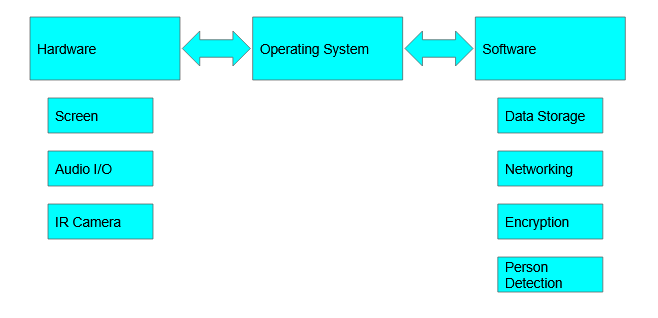
\includegraphics{UML}
\caption{UML Diagram}
\end{figure}

\section{Design Stakeholders and Their Concerns}
The client, D. Kevin McGrath, is the only stakeholder for this project. The scope of the Smart Home Intercom is a proof of concept of the system which will be used within a home. In terms of cost, the client requires each unit of the system be roughly \$200 per unit or less. The system should require little setup and be able to stream video and audio between two nodes. There is a strong emphasis on the security of the system: it cannot connect to outside networks and must encrypt audio and video streamed between nodes. At least four nodes should be able to be supported, and additional nodes should be easy to add.

\section{Design Viewpoints}

\subsection{Hardware}
\subsubsection{Video Display Hardware}
The system will use a 7" display to show the UI and incoming/outgoing video feed during video calls.
The display will connect to an adapter board with a ribbon cable, and Raspberry Pi 3 (RPi3) then connects to the adapter board with another ribbon cable and 2 jumper wires connected to the respective pins.
Jumper wire one is connected to PIN 2 on the RPi3, and the 5V PIN on the adapter board. Jumper wire two is connected to PIN 6 on the RPi3, and the GND PIN on the adapter board. Then the display, adapter board, and RPi3 are housed in a wall mountable case. The display hardware is plug and play with the RPi3 so there is no additional configuration required for the display to show the UI, however, incoming/outgoing video feeds need to be handled by additional software before being able to be displayed.

\subsubsection{Audio I/O}
Audio I/O for the Smart Home Intercom project will involve using a compatible audio hat with the Raspberry Pi 3 to get quality audio to be streamed between nodes. Since this is a core part of the project and will need to be integrated with almost every other design piece, this should be implemented as early as possible. The audio I/O can be tested by recording audio input through the mic, then playing it out through speakers. Doing this will give a good estimate as to the quality of the audio when it is integrated with the rest of the project. Eventually, the audio will have to be encrypted then streamed to another device, which may affect its quality so audio I/O will need to be tested thoroughly after multiple nodes are setup to stream this data. In order to process audio data on a node, a script will need to be implemented that will activate when a user wants to make a call in order to activate the microphone and speakers so that audio can be recorded and streamed. The audio data will not be stored at any point, so it should be immediately encrypted and streamed after recording.

\subsection{Software}
\subsubsection{Operating System}
Selecting the operating system came down to familiarity and ability to control the system as would be needed. Given this, Raspbian is ideal. There are two versions of Raspbian in release, Stretch and Stretch Lite. While Stretch is fine as an out of the box operating system and does not require much work, Stretch Lite offers customizability as well as being extremely lightweight. Given that the device should be locked into the Smart Home Intercom System software, Stretch Lite is only command line and it is possible to set a shutdown OnExit() via Qt. Because of the similarity between packages, Stretch will be used to develop on and as soon as all packages that will be required are known, Stretch Lite will be implemented instead of Stretch. Should Stretch Lite be unable to implement all packages that are required, a purposefully modified version of Stretch can potentially be used. It would require removing packages from Stretch instead of building packages up with use of Stretch Lite. The development timeline for OS is skewed due to networking and the user interface taking precedence, it will be the first thing implemented and one of the last things worked on.

\subsubsection{Data Management}
Data will be managed by using flat files and system calls to read and write from or to them. Since this is already an integral part of the system, no setup or external hardware/software will be necessary beyond an operating system. This is a highly reliable way of storing data, so any testing would involve ensuring the integrity of the data being written to files and preventing harmful data from interfering with any part of the system. Since data will have to be stored regarding the location of a person, testing will need to be done to ensure the right association between person and room is made and that this information can be reliably retrieved. Detailed errors will also be logged (beyond what the user would immediately see) for troubleshooting purposes, and this can be tested by purposefully triggering bugs to see if errors log correctly.

\subsubsection{Networking}
The networking portion will use the Qt 5.0 network module for encapsulating application data and Better Approach to Mobile Adhoc Networking advanced (batman-adv) will be responsible for communication between units. For a smooth transition and knowledge of these processes working correctly, implementation will first be at the application level with Qt 5.0 by using the backbone of a router and then one node will be transitioned to batman-adv and left to communicate with the device still on a router. Upon successful completion of that task, the device left on the router will be transitioned to batman-adv and the router will be powered off in hopes that the devices remain connected. A script will be created to mimic settings that need to be input for batman-adv to work and one device will be hard reset and then run with the script. The device that was just reset should connect to the other device without any issues.

\subsubsection{Network Encryption}
To protect users video and audio feeds an encryption method needs to be implemented at the application level.
Salsa20 satisfies this requirement and works in conjunction with VLC by encrypting the video/audio feed as it streams. The encryption method has multiple libraries available in various programming languages like C++ and Java that can be run on the RPi3.
To test that the video and/or audio feed between two nodes is correctly encrypted, the feed can be intercepted by a third node, and if the video and audio stream is unable to be viewed by that node then the feed is correctly encrypted.

\subsubsection{Person Detection}
Person detection will involve identifying when a person is in a room in order to log that this person was in a certain location. This will be developed using software libraries for facial recognition, such as OpenCV, and potentially using the IR capabilities of the camera as well. In order to test this system, a program would wait for someone to enter the frame of the camera (could be done with motion sensing or IR detection) and then attempt to recognize their face. If successful, it should log the results to a file to keep track of where this person is. Person detection can be implemented almost completely independently of the rest of the system, so this should be completed before winter term begins or within the first week. Since person detection will affect when the system turns itself on, a program will need to run to be developed to wake the system up when this occurs.

\subsection{Interface}
\subsubsection{User Interface}
The user interface will be implemented using Qt 5.0. Qt 5.0 is opensource and has an ample amount of examples online. Development will be done using a Debian Stretch virtual machine to assure it can be ported correctly to the Raspbian Stretch operating system on the Raspberry Pi 3. The first step with the user interface is using the network module in some capacity to be able to test the networking approaches. From that point, development of the actual user interface can begin. The user interface should contain the following options: room selection, camera on/off, page and volume. There should be a video box that pops up on the screen and a menu to switch user modes and tweak user interface options, like brightness and contrast. In administrator mode there should be a way to monitor select devices and use the system in broadcast mode.

\subsubsection{Video Display Software}
VLC will be used to handle the incoming/outgoing video feeds before being displayed on the screen.
Installation of the software onto the system is done through a package, because the system is using Raspbian as the OS and VLC supports Debian Linux distributions.
The software does not need additional configuration to be able to playback video, however, it does need to be configured to be able to stream video feed between two nodes.
Configuration of streaming video is done by setting the first node to stream the video feed out, then the second node connects to and displays the stream with VLC using the IP address of the first node.
The configurations are required to be set on both nodes, so that the video feeds of both nodes can be displayed on each other, and must be set every time a video call is attempted to be established.

\section{Summary}
Although requirements and development strategies will inevitably change during implementation, this document should be roughly adhered to and updated with relevant information. The parts of the system that are the most integral, such as video and audio streaming, should be implemented early in winter term to ensure the other parts can be built on top of this. Parts of the project that can operate independently of others, such as person detection, should also be implemented earlier. 

\end{document}

